
%The goal of this Chapter is to show how \name can improve the traditional top-down analysis method. Usually, researchers start from a deep comprehension of the theoretical problem and draw a model of the system. This model is exploited to formulate hypothesis and even if further knowledge about the implementation experience may support this method, this approach is traditionally top-down. Section \ref{sec:empirical-research} shows there is a lack in Computer Science about system evaluation. However, when the subject of the research are complex system, it is hard to formulate and prove hypothesis that are only based on he knowledge of the model and empirical evaluation becomes useful.

In this chapter we present an evaluation of \name Baselines (See Chapter \ref{sec:baselines}) in order to demonstrate how \name can extend the traditional hypothesis-based research, towards the Systematic Comparative Research approach we introduced in Chapter \ref{chap:problem-settings}. In section \ref{sec:experiment-design} we introduce the method we follow to design experiment. Moreover, we detail the assumptions we formulate and the design choices behind two sets of experiments executed on \name Baselines: SOAK Tests in Subsection \ref{sec:soak-es} and Step Response Stress test in Subsection \ref{sec:step-es}. Finally, we present the experiment results respectively for SOAK test in Section \ref{sec:soakres} and for the Step Response Test in Section \ref{sec:stressres}.

The aim of SOAK tests is showing the problem that are in the traditional top-down analysis of complex software systems like RSP Engines. Even for simple hypothesis. Consequently the evaluation with SOAK Tests demonstrates that we need \namens. The Step-Response tests are designed with the goal to show \name potential, and provide a simple case of analysis inspired by the Systematic Comparative Research Approach.

\section{Experiment Design}\label{sec:experiment-design}

Experiment design (ED) means design our experiment in order to prove or refute one or more hypothesis, evidencing the behaviour of the system in a controlled and well defined execution environment. ED starts with some assumptions, which compose the  Experimental Setting. Researchers formulate hypothesis on the base of these assumptions, Figure \ref{fig:experiment-design} summarises the collocation of ED within the Top-down approach.

\begin{figure}[tbh]
  \centering
	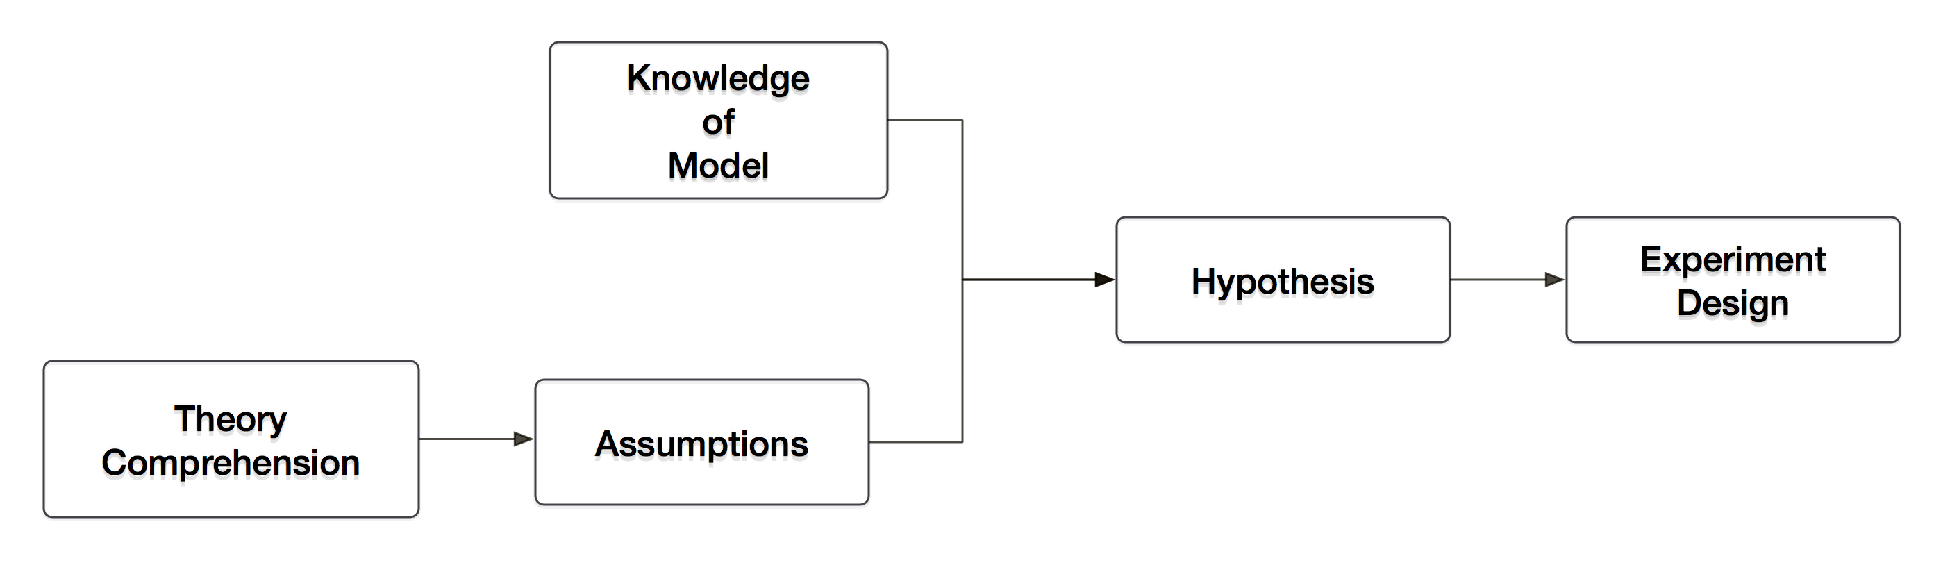
\includegraphics[width=\linewidth]{images/experiment-design}
	\caption{Traditional Experiment design workflow} 
  	\label{fig:experiment-design}
\end{figure}

From a theoretical point of view we decide to study RSP Engine facing their nature of dynamic system. (see Section \ref{sec:sfp}). Experiment design requires to point out which variable are observed. We simplify the study analysing their behaviour in term of Latency and Memory, which is the minimal meaningful measurement set for an RSP Engine (Chapter \ref{chap:heaven}).

In Chapter \ref{chap:heaven} we describe the experiment tuple: $<\mathcal{D}, \mathcal{T},\mathcal{E}, \mathcal{Q}>$ , where briefly:
\begin{itemize}
\item $\mathcal{E}$ is the RSP Engine
\item $\mathcal{D}$ is the Dataset 
\item $\mathcal{T}$ is the Ontology
\item $\mathcal{Q}$ is the Query that $\mathcal{E}$ continuously answers.
\end{itemize}

In this section we present our choices about the four elements that compose an experiment, upon which the evaluation is built

\subsection{Engine $\mathcal{E}$}

%. Top-Down investigations are commonly hard, and they become even harder for commercial solutions.
The architecture complexity of mature RSP Engines like the C-SPARQL Engine or CQELS is high, and it can not be easily faced in order formulate hypothesis of comparison. However, the purpose of this evaluation is showing how \name can improve the research of RSP Engine. Thus, we can simplify the research survey evaluating less complex systems. To this extent we design and implement the Baselines (Section \ref{sec:baselines}) and we evaluate them as the RSP Engines $\mathcal{E}$ subject of our experiments. 

In Chapter \ref{chap:problem-settings} we describe which requirements guarantee that an RSP Engine is a baselines: Simplicity, Elementarily, Relevance and Eligibility (SERE properties) legitimate the evaluation. Thus, they can be considered as a simple term of comparison for further research on Stream Reasoning systems and this investigation can be followed as a guideline.
 
The four baselines differ for two characteristics: RDF Stream Model and Reasoning architecture. The Table \ref{tab:baselines-names} summarises these few but well determined differences, naming the four baselines for the evaluation:\begin{table}[htb]
\scriptsize
\centering
\begin{tabular}{c|cc} % creating eight columns
	\hline
         & Naive & Incremental\\
	\hline
	Graph        &  GN      & GI\\
	Triple   &  TN   & TI\\
	\hline % inserts single-
\end{tabular}
\caption{Naming convention of the four baselines, further details in Section \ref{sec:baselines}}
\label{tab:baselines-names}
\end{table}

\noindent Among these four configurations we can formulate simple hypothesis, stating which approach is better then an other one within an experiment. Notice that we have a complete model of the baseline systems and we also know many implementation details that can help during the analysis. We can exploit the know-how about their internal mechanisms, described in Section \ref{sec:baselines-impl}, to lead our analysis from hypothesis formulation towards empirical results. 

\subsection{Dataset $\mathcal{D}$ and Ontology $\mathcal{T}$}\label{sec:dataset}

\noindent The Dataset  $\mathcal{D}$ and the Ontology $\mathcal{T}$ must be chosen to ensure baselines Simplicity, as stated in Section \ref{sec:baselines}. 

The RDF Streams (details in Section \ref{sec:rdfstream}) $\mathcal{D}$ used in the experiments are obtained streaming in different ways the data generated with LUBM  \cite{Guo2005}. Consequently we chose LUBM ontology\footnote{http://swat.cse.lehigh.edu/onto/univ-bench.owl} as $\mathcal{T}$ for all the experiment. We assume that the ontology does not change over time, therefore the materialisation of $\mathcal{T}$ is computed before starting the experiment and the RSP engine does not have to perform this task. 

It is worth to discuss the choice of using data from LUBM (Section \ref{sec:lubm}) rather than SRbench or LSbench. The first one has data, which are not adequate for the experiments, since they do not require any reasoning. The SRbench data, on the contrary, requires reasoning, but, being real-data, do not have the possibility to be scaled up and down. Further details on SRbench and LSBench can be found in Section \ref{sec:lsbench}. Moreover, this choice is in line with previous works on Stream Reasoning \cite{DBLP:conf/semweb/UrbaniMJHB13}. 

Being LUBM static data, we exploit the \textit{RDF2RDFStream} component of the \textsc{Test Stand} that takes care to adapt the data generate by LUBM to a streaming scenario (see Section \ref{sec:streamer-impl}). \textit{RDF2RDFStream} is responsible to build $\mathcal{D}$ w.r.t. $\mathcal{T}$, scaling both in terms of dimension of the dataset and the reasoning effort. The component can be set up to obtain an RDFStream where the number of triples with the same timestamps follows a given distribution. %Section \ref{sec:streamer-impl} contains all the details about the implementation and the usage of this particular \textsc{Streamer}. %e' veramente il timestamp quello?

\subsection{Query $\mathcal{Q}$}\label{sec:query}
 
The the query $\mathcal{Q}$ used in our experiment depends on the reasoning approach of the RSP Engine in use. Actually, all  experiments uses variants of the basic identity query that continuously asks for the materialisation of the current sliding window $\omega$, which differ from the sliding factor $\beta$.\\

\begin{center}
\raggedright
REGISTER QUERY Q AS \\
SELECT ?s ?p ?o \\
FROM STREAM S [RANGE $\omega$ STEP $\beta$]\\
WHERE {?s ?p ?o}\\
UNDER $\rho$DF ENTAILMENT REGIME
\label{code:query}

\end{center}
Query: \ref{code:query}: Query $\mathcal{Q}$ registered to the \name Baselines.\\


The Baseline GN and TN exploit the Naive Reasoning approach and thus the query \ref{code:query} is implemented in order to output the snapshot of the entire window at each slide of the window. On the other hand, the Baselines GI and TI exploit the Incremental Reasoning approach and thus implement the query \ref{code:query} in order to output the ir-streams at each window slide.

The entailment regime of the RSP Engines influence performances. For this reason we take $\rho$DF  \cite{DBLP:conf/esws/MunozPG07} as their entailment regime, because several works in the field \cite{DBLP:conf/semweb/UrbaniMJHB13, Liu:2014:ERS:2567948.2577323} choose this as the minimal meaningful task for a Stream Reasoner. In particular, $\rho$DF is the RDF-S fragment that reduces complexity while preserving the normative semantics and core functionalities.

%We describe in details the content of the SOAK (Section \ref{sec:soak-es}) and the Step Response tests (Section \ref{sec:step-es}), providing a lecture key for the experiment results.

\section{Experiment Set-Up}

The \textit{RDF2RDFStream} allows to control the triple distribution in the RDFStream, thus it is possible to build experiment with different input RDF Stream. We design set of SOAK Tests to evaluate the Baselines, which can evidence how as baseline behaves over very long executions providing an image of the RSP Engine dynamics. Moreover, in order to show \name potential, we design a small set of Stress Test, which belongs to the Step Response subcategory. In summary:

\begin{itemize}
\item \textbf{SOAK}: the number of contemporary triple in the RDFStream does not change during the experiment.
\item \textbf{Step Response} the number of contemporary triple in the RDF Stream does not changes for a certain period of time that guarantees the system to reach a stable condition, then it suddenly increase or decrease. The number of triple in the RDF Stream does not changes any more, giving to the system the possibility to reach the stability again.
\end{itemize}

Experiments are executed on \name Baselines and the queries registered to them variate for the size of the sliding window $\omega$ . In particular, we use windows in which $\omega$ is an integer multiple of the slide parameter $\beta$ of the window, i.e., it holds that $\omega = \beta * N$. In other words, $N$ is the number of \textsc{CTEvents} that the window contain. 

Moreover, Section \ref{sec:baselines-impl} shows how the proposed baselines take advantage of the ability of Esper to be temporally controlled by an external agent\footnote{\url{http://esper.sourceforge.net/esper-0.7.5/doc/reference/en/html_single/index.html#api-controlling-time}} by sending time-keeping events to synchronise the internal time flow. All the triples in the \textit{CTEvent} are consider contemporary by the baselines and each \textit{CTEvent} can be seen as a proxy for the timing event. Together with the \textit{RDF2RDFStream} is possible to estimate the content of the current window in terms of number of RDF Triples in any moment of the experiment.

All experiment are execute 10 times to reduce the presence of the outlier.

The following subsections contain further details about the two test sets, respectively in Subsection \ref{sec:soak-es} for SOAK Test and in Subsection \ref{sec:step-es} for Step Response tests.

\subsection{SOAK: Tests and Hypothesis}\label{sec:soak-es}

Soak testing show the system dynamics, injecting to the RSP Engine in use a constant and continuous input flow (see Section \ref{sec:software-testing}) . We control the number of contemporary triples in the RDF Stream trough the \textit{RDF2RDFStream} module. %Moreover, Section \ref{sec:query} describe how we variates the query between experiments.

SOAK Experiment are 30000 CTEvent long, each one of a fixed size, which depend on the specific experiment. Unlikely, it is not possible to foretell how many events are required in to reach the Steady State condition for each variable involved, especially memory. The Experiment Results show this in detail in Section \ref{sec:soakres}. Multiple attempts and empirical evaluation are the only way to set up the correct duration.

\begin{table}[htb]
\centering
\normalsize
 \begin{tabular}{l| ccccc}
	  	\hline
		\textsc{CTEvent}  &\multicolumn{5}{c}{Number of Slot}  \\
		Size  & 1 & 10 & 100 & 1000&10000 \\
		\hline	
		1 & 1& 10 & 100 & 1000&10000 \\
		10  & 10 & 100 & 1000&10000 \\
		100 & 100&1000&10000  \\
		1000 &1000 & 10000 \\
		10000&10000  \\
		\hline 
	\end{tabular}
	
	 \vspace{10pt}
	\caption{The number of triples in the window during the fifteen SOAK tests as a function of the Window size (in terms of $N$) and of the triples in each \textsc{CTEvent}.}
	\label{tab:soaktests}
\end{table}

\begin{table}[htb]
	\centering
	\normalsize
	\begin{tabular}{l | ccccc} % creating eight columns
	  	\hline
		Triple in & \multicolumn{5}{c}{Number of Slots}  \\
		Window  & 1 & 10 & 100 & 1000&10000\\
		\hline
		1  	 & 1\\
		10   & 10  & 1 \\
		100  & 100 & 10 & 1\\
		1000 & 1000& 100& 10& 1\\
		10000& 10000 & 1000& 100& 10& 1\\
		\hline % inserts single-line
	 \end{tabular}
	\caption{The number of triples in a \textsc{CTEvent} during the fifteen SOAK tests as a function of the Window size (in terms of $N$) and of the total triples in the active window, assuming one and only one \textsc{CTEvent} per slot.}
	\label{tab:soaktests-alt}
\end{table}

Table \ref{tab:soaktests} presents the fifteen SOAK tests we run for each baseline presented in Table \ref{tab:baselines-names}. The columns of the table are the different window sizes measured in terms of the values assumed by $N$ (see Section \ref{sec:query}).  Being $\beta=$ 100 ms., they correspond to a window that spans 100 ms., 1 sec., 10 sec. and 100 sec.. The rows are the different number of triples in each \textit{CTEvent} sent by the \textsc{RDF2RDFStream} to $\mathcal{E}$.% Notably, for all of them, we checked that $\mathcal{E}$ is responsive for the whole duration of the experiment. 

Table \ref{tab:soaktests-alt} is an alternative layout where the columns of the table still contain the different window sizes measured in terms of the values assumed by the number of slots $N$, while the rows are the different number of triples in the active window. The alternative disposal allows to highlight the windows dimension, focusing on the element which actually influences the reasoning.

Following the traditional research method, we formulate two naive hypothesis based on the knowledge we have of the easiest RSP Engine Model (detailed in Section \ref{sec:baselines}) . The hypothesis to verify with SOAK experiments are:
\begin{itemize}
\item \textbf{HP.1} The Incremental reasoning approach is always better then the naive one.
\item \textbf{HP.2} The Triple-based model for RDFStream is always better then the Graph-based one.
\end{itemize}

%Notice that the goal of this evaluation is to show how \name helps RSP Engine analysis trough empirical research. Hypothesis verification and top-down analysis are the subject of our investigation, while our research question is:  "\textit{Can an engine test stands, together with queries, datasets and methods, support Systematic Comparative Research Approach for Stream Reasoning?}" %"Needs the Stream Reasoning research field a Test Stand like \name to investigate RSP Engines and sustain the research of such system with an Systematic Comparative Approach?"

\subsection{Step Response Tests}\label{sec:step-es}

Step Response testing allow to see how the system reacts to a sudden changing in the input condition (see Section \ref{sec:software-testing}). They are related to SOAK test, because they allow to study deeply the initial warm-up phase of the system. This set of experiments evidence the different responses of an RSP Engine if we move form an input condition to another instead of starting from scratch.

We design the step experiments concatenating two with total length of 400000 events, which means hours of execution for the system. For this reason we investigate only few configuration, all with 10  window slot size for all the four baselines. Table \ref{tab:steptests} summarises the step experiment set-up, where the step is positioned at the half of the execution, 20000 events.
\begin{table}[htb]
\centering
 \begin{tabular}{c|c|c}
	  	\hline
	  	&\multicolumn{2}{c}{CTEvent size}  \\
		Window Size & Initial Size & Final Size\\
		\hline
		\hline
		 10 & 10 & 100\\
		  10 & 100 & 1000\\
		 10 & 10 & 1000\\
		\hline 
 \end{tabular}
 \caption{}
\label{tab:steptests}
\end{table}

We do not formulate hypothesis for Step experiments. The purpose of this test set is to show \name capabilities and not to offers a deep understating of the baselines. However, we comment the results evidencing the finding in the sections below.

\subsection{Execution Environment}\label{sec:execution-environment}

Before presenting experiment result a brief description of the execution environment is required. All experiment are executed exploiting a dedicated machine, an iMac mid-2011 with 12GB RAM and 3.6 Ghz of a Intel i5 64 Bit, which run OS X 10.10.2 Yosemite,. Since \name is developed with Java 7\footnote{http://www.oracle.com/technetwork/java/javase/javase7locales-334809.html}, we use the versione 1.7.0.71 of the JVM.
The execution happens in a controlled environment, which tries to reduce the number of disturbing elements like network, graphical interface and other running processes.

\section{SOAK Test Evaluation Results}\label{sec:soakres}

In this section we analyse the results of the SOAK Test experiments, exploiting the investigation stack presented in Chapter \ref{chap:heaven}. The analysis goes through the four levels of the stack, with the aim of confirming or refusing the hypothesis presented above, in Section \ref{sec:soak-es}. 

The content of this section is organised as follow: Firstly we present, in Subsection \ref{sec:eval-ssib} the output of the \textit{Steady State Identification} Block. Subsection \ref{sec:eval-level0} presents the results obtained at Level 0, the dashboard visualisation.  Subsection \ref{sec:eval-level1} provided a qualitative comparison for Latency and Memory, built trough Level 1 tools. Subsection \ref{sec:eval-level2} contains example of pattern identification (Level 2). Finally in Subsection \ref{sec:eval-level3} we include some examples of the Level 3 intra-experiment comparison techniques, while example of inter-experiment comparisons can be found in Section \ref{sec:stressres} w.r.t Step Response tests.


\subsection{Steady State Identification Block Results}\label{sec:eval-ssib}

The \textit{Steady State Identification} (SSI) Block, as reported in Chapter \ref{chap:implementation-experience}, annotates the averaged raw data received by the \textit{Pre-Processing} Block, indicating which variable has reached a Steady State condition for an experiment. Table \ref{tab:ss-cond} contains all the results the SSI Block, distinguishing between latency and memory for each variables

\begin{table}[htb]
\centering
\scriptsize
 \begin{tabular}{c|c|c|cc|cc|cc|cc}
	  	\hline
	  	&&&\multicolumn{8}{c}{Steady State Condition Identification Result}  \\
	  	&CTEvent&&\multicolumn{2}{c}{GN}|&\multicolumn{2}{c}{GI}|&\multicolumn{2}{c}{TN}|&\multicolumn{2}{c}{TI}  \\
	  	EN&Size& Slot Num.&Lat&Mem&Lat&Mem&Lat&Mem&Lat&Mem  \\
		\hline
		\hline
		 1&1&1&Yes&Yes&Yes&No&Yes&Yes&Yes&Yes\\
		 2&10&1&Yes&Yes&Yes&Yes&Yes&Yes&Yes&Yes\\
		 3&100&1&Yes&Yes&Yes&Yes&Yes&Yes&Yes&Yes\\
		 4&1000&1&Yes&Yes&Yes&Yes&Yes&Yes&Yes&Yes\\
		 5&10000&1&NA&NA&NA&NA&NA&NA&NA&NA\\
		 6&1&10&Yes&Yes&Yes&Yes&Yes&Yes&Yes&Yes\\
		 7&10&10&Yes&Yes&Yes&Yes&Yes&Yes&Yes&Yes\\
		 8&100&10&Yes&No&Yes&No&Yes&No&Yes&No\\
		 9&1000&10&Yes&Yes&Yes&Yes&Yes&Yes&Yes&Yes\\
		 10&1&100&Yes&No&Yes&Yes&Yes&Yes&Yes&Yes\\
		 11&10&100&Yes&No&Yes&No&Yes&No&Yes&No\\
		 12&100&100&Yes&Yes&Yes&Yes&Yes&Yes&Yes&Yes\\
		 13&1&1000&Yes&No&Yes&No&Yes&No&Yes&No\\
		 14&10&1000&Yes&Yes&Yes&Yes&Yes&Yes&Yes&Yes\\
		 15&1&10000&Yes&Yes&Yes&Yes&Yes&Yes&Yes&Yes\\

		\hline 
 \end{tabular}
 \caption{}
\label{tab:ss-cond}
\end{table}

All the SOAK Experiments reach the Steady State condition for latency, but some of them did not for memory. Notice in particular that experiment with CTEvent Size = 1000 and a Number of slot greater than 1 (8, 11,13) did not reach memory Steady State. Moreover Experiment number 5,  with the CT Event Size = 10000 a Slot Number = 1 did not terminate correctly due to an execution error. The reader please ignore the results of this experiment, which are not actually part of our evaluation.

\subsection{Level 0 - Dashboards}\label{sec:eval-level0}

\begin{figure}[tbh]
	\centering
	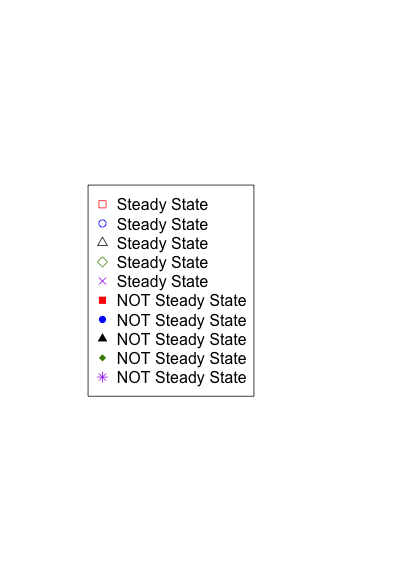
\includegraphics[width=0.25\linewidth]{images/dashboard-legend}	
	\caption{Dashboard Legend} 
	\label{fig:dashboard-legend}
\end{figure}

The SOAK test results analysis starts with the high level dashboard view. Each dashboard presented is composed by two chart which shows in different form the relation between the different four baselines. Dashboard legend is fixed for all the following charts and reported in Figure \ref{fig:dashboard-legend}.

\textbf{Dashboard One - Fixed Size \textsc{CTEvent} = 1} - 

\begin{figure}[htb]
	\centering
	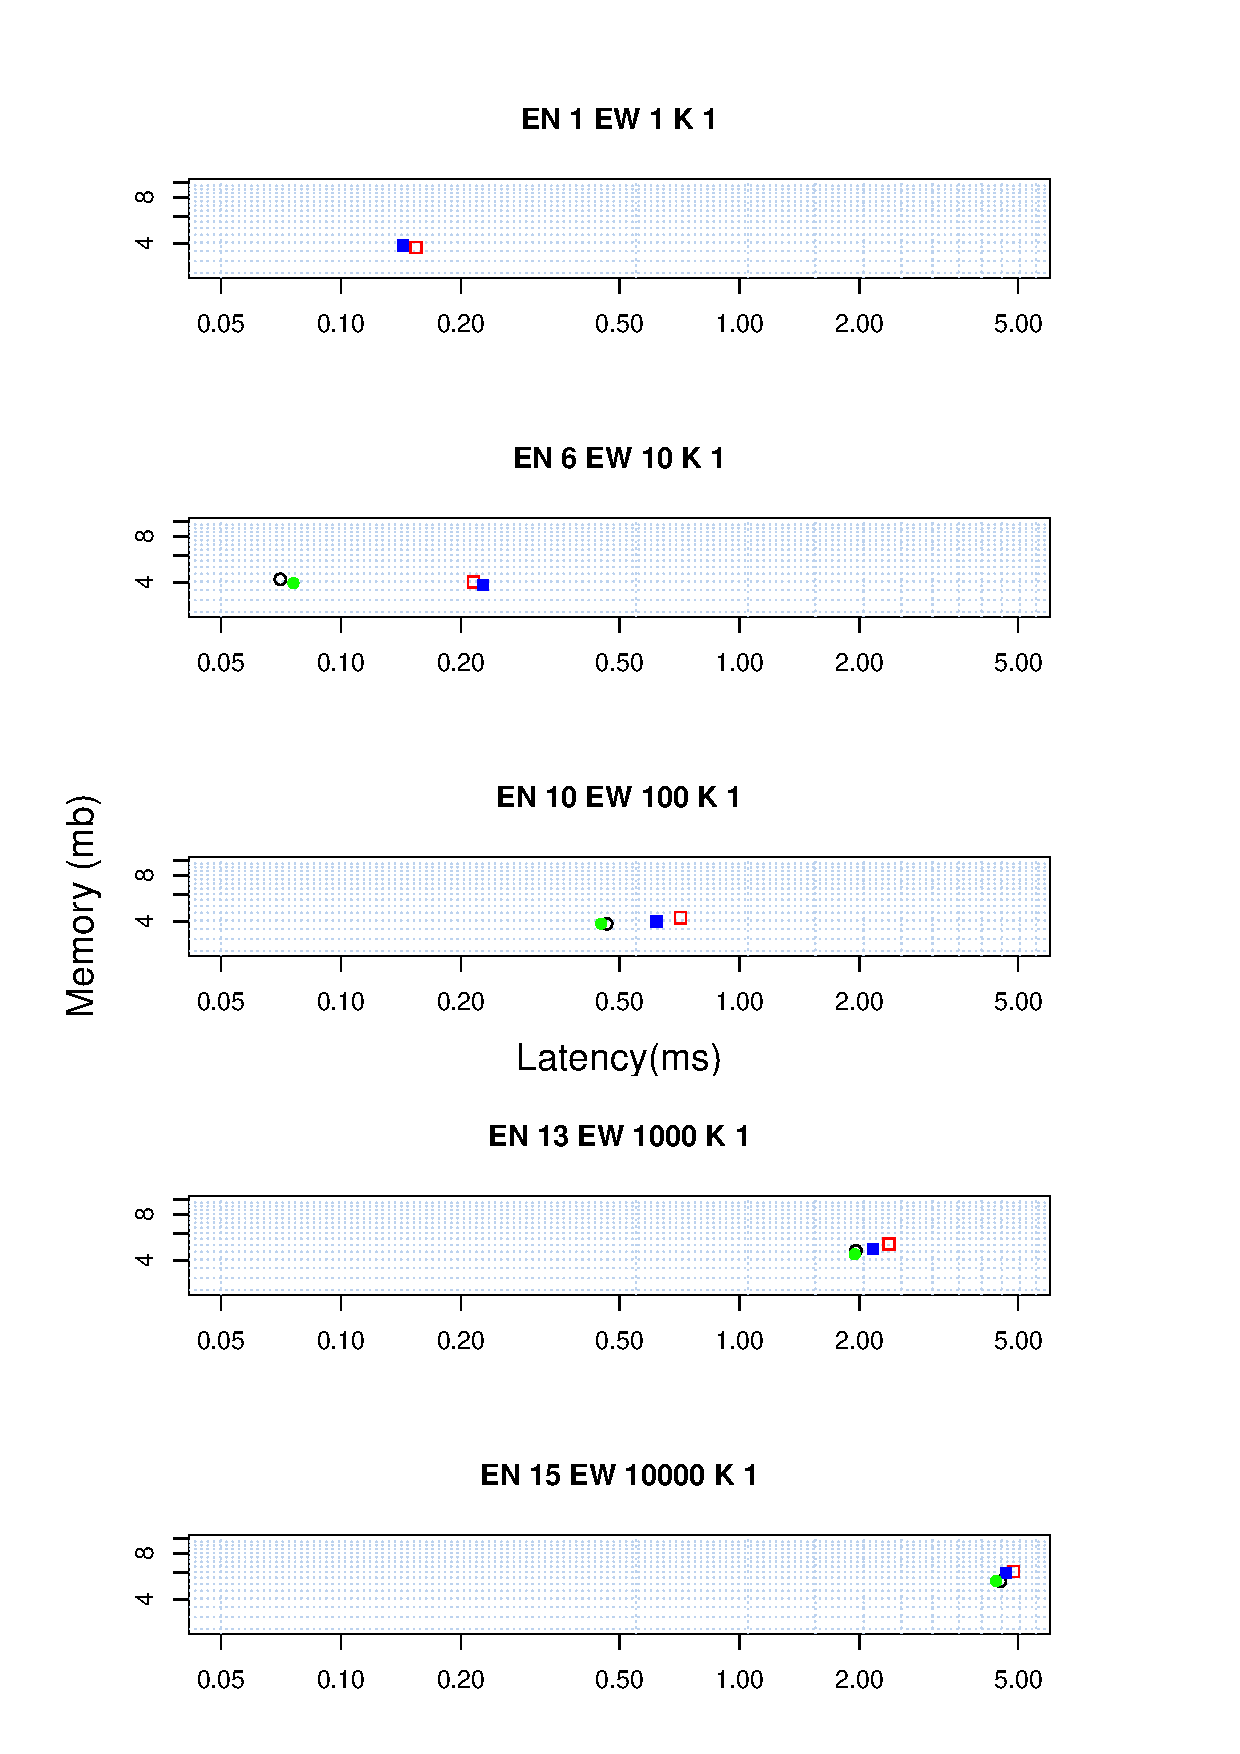
\includegraphics[width=0.90\linewidth]{images/dashboard-1-split}	
	\caption{Dashboard One - K=1 Split} 
	\label{fig:result_dashboard_ka}
\end{figure}

\begin{figure}[htb]
	\centering
	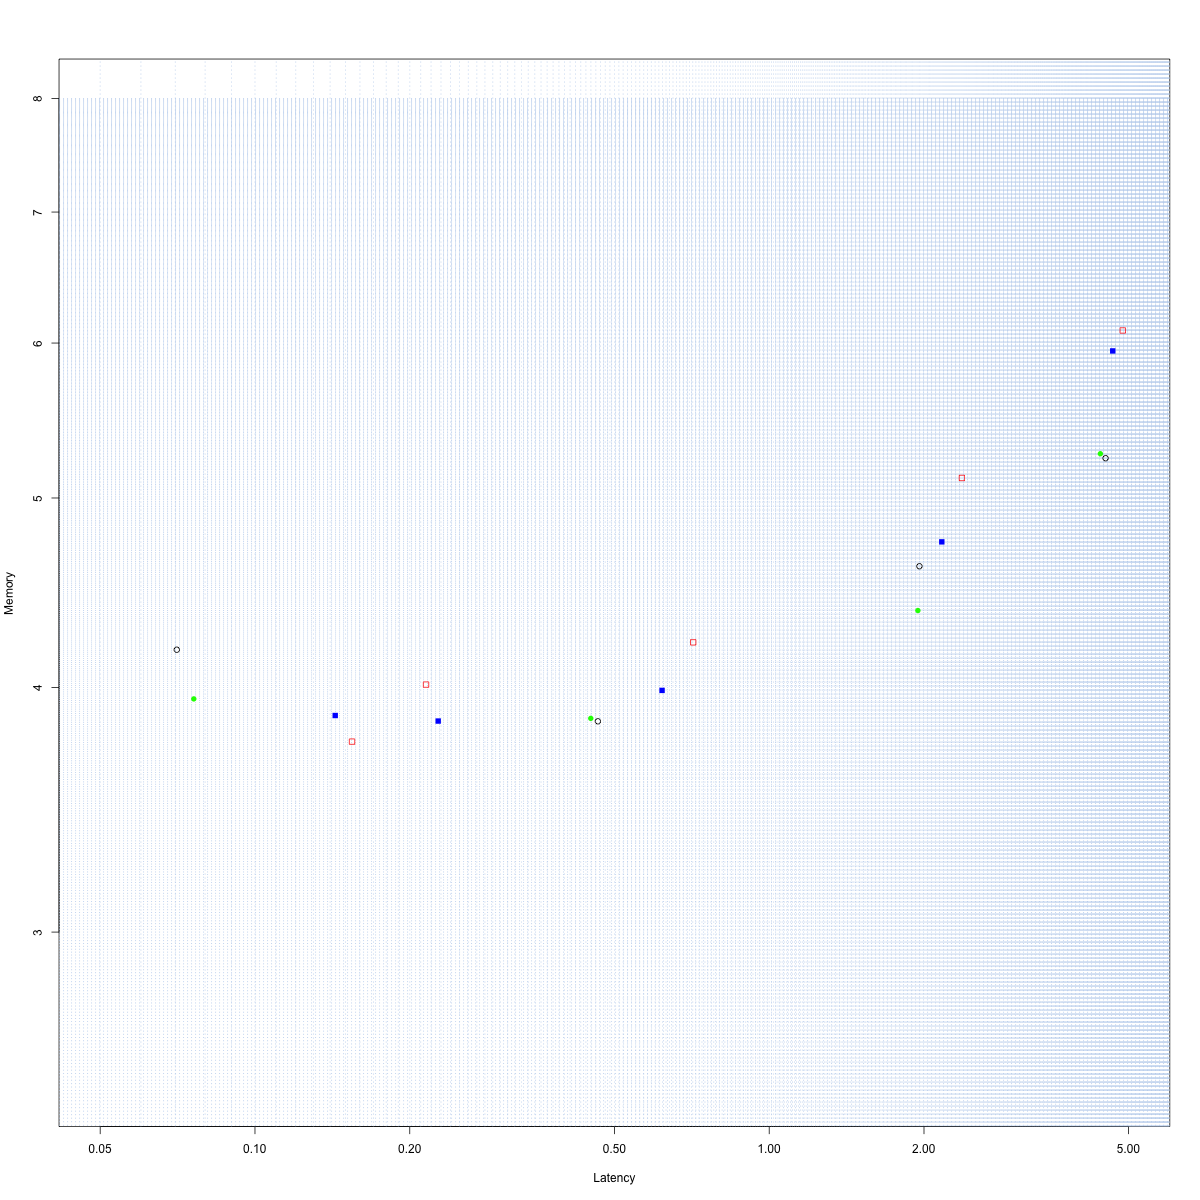
\includegraphics[width=0.90\linewidth]{images/dashboard-1}	
	\caption{Dashboard One - K=1 Multiplot} 
	\label{fig:result_dashboard_kb}
\end{figure}

%and \ref{fig:result_dashboard_kb}
Figures \ref{fig:result_dashboard_ka} shows how the behaviour of the four Baselines changes between a set of experiments which has a fixed CTEvent Size = 1 Triple and variates the number of Slot in the active window, from 1 (Tumbling) to 10000. Comparing to the experiment layouts of Table \ref{tab:soaktests-alt}. Fixing the \textsc{CTEvent} size while the Number of slot is changing means moving on the table diagonals, if \textsc{CTEvent} size = 1 indicates the latest one.

In Figure \ref{fig:result_dashboard_ka} we can appreciate that increasing the number of slots in the active window, and thus the window size (in terms of triple), all the baselines have a worsening in terms of Latency. The Baselines which exploits the Incremental reasoning approach, GI and TI, are not represented in the Figure when the number of slides is equal to one (Tumbling window of only one triple), because their latency it too small to be represented in this scale. Increasing the number of slot, GI and TI have the major worsening in term of latency w.r.t GN and TN. Actually they do not became worse, but when the number of slots became high (10000) and the variation is about 2/10000,  the Incremental approach is at least comparable with the naive one. We can assume that with an higher number of slot, GI and TI can overtaking  GN and TN.

Observing Figure \ref{fig:result_dashboard_kb}, which shows all the experiment within a single image,we can also individuate the worsening for the memory consumption. A first obvious insight may be that \textit{Bigger problem requires in general more resources}. Another insight regards the difference in term of latency, the x-asis, between the different baselines.

Dashboard One confirms Hypothesis [Hp.1]: the incremental approach has better latency and memory performance than the naive one. For [Hp.2] the confirmation is partial. The latest results in Figures \ref{fig:result_dashboard_ka} shows that the Memory Consumption strictly depends on the reasoning approach and the Graph-based stream my be better than the Triple-based one. For Latency [Hp.2] is confirmed for the experiment with a big window, while the smaller one may works better with a Graph-Based stream.


\textbf{Dashboard Two - Fixed Number of Slot = 10}


\begin{figure}[htb]
	\centering
	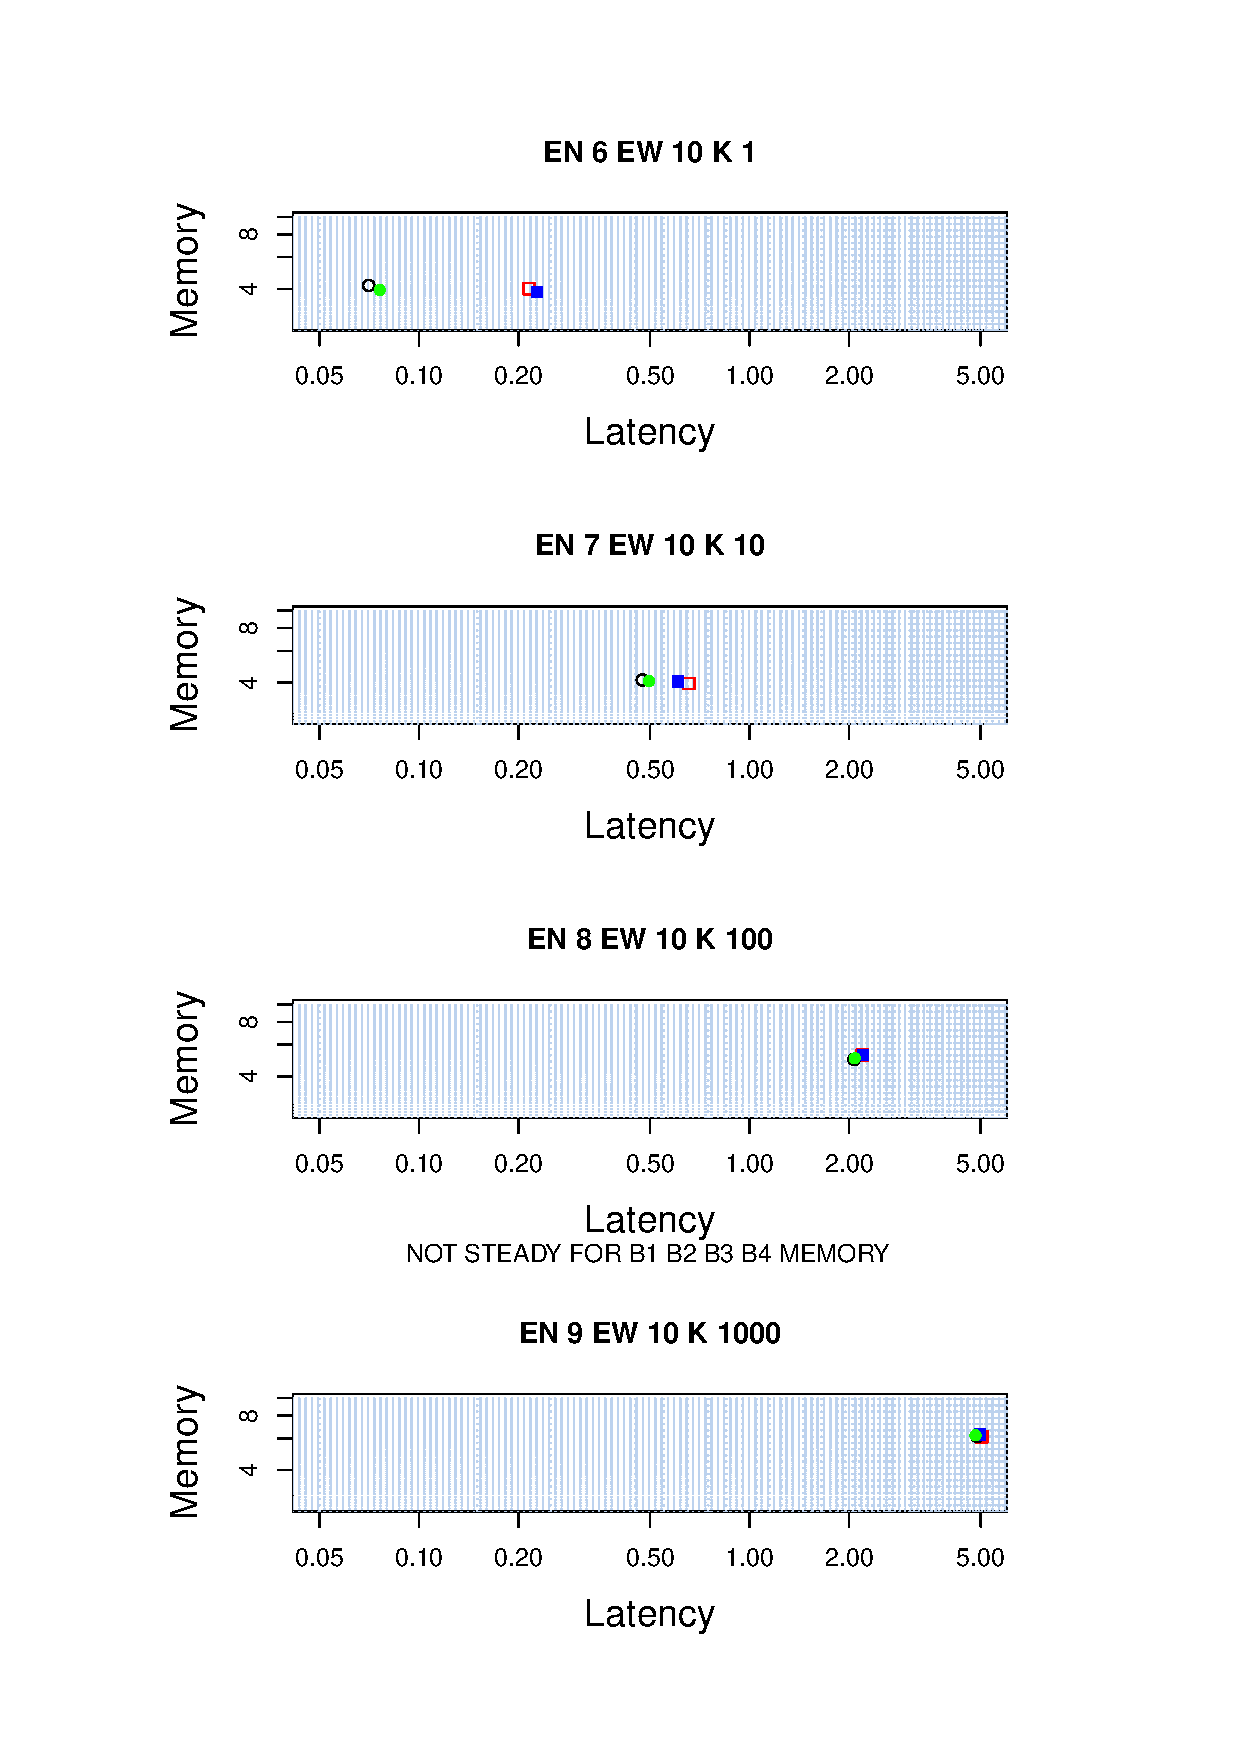
\includegraphics[width=0.90\linewidth]{images/dashboard-2-split}	
	\caption{Dashboard Two - EW=10 Split} 
	\label{fig:result_dashboard_ewa}
\end{figure}

\begin{figure}[htb]
	\centering
	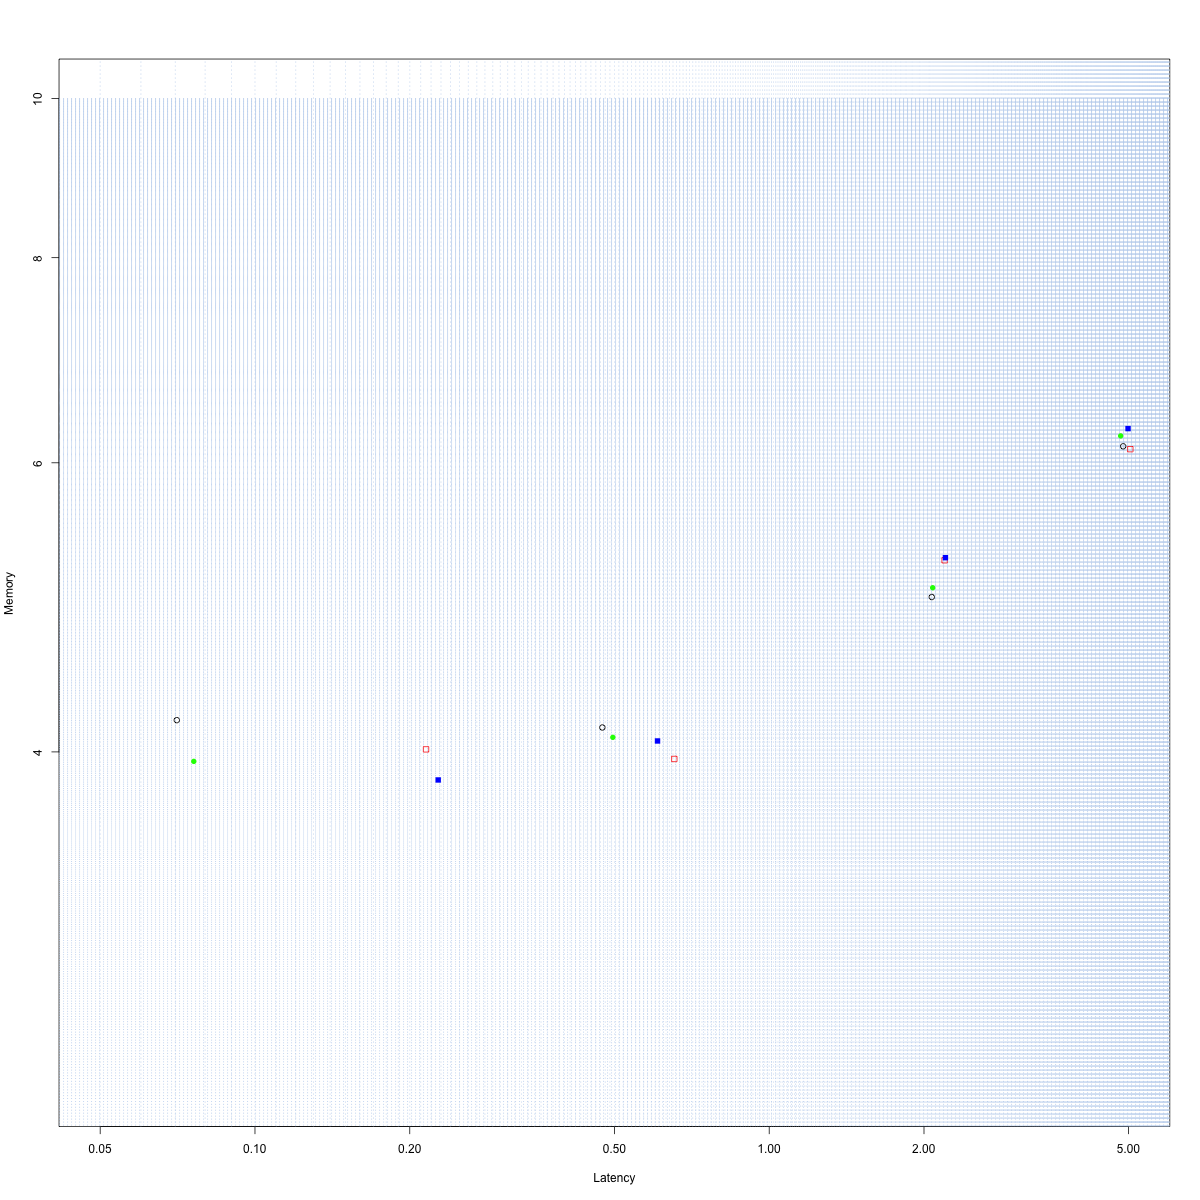
\includegraphics[width=0.90\linewidth]{images/dashboard-2}	
	\caption{Dashboard Two - EW=10 Multiplot} 
	\label{fig:result_dashboard_ewb}
\end{figure}


Figure \ref{fig:result_dashboard_ewa} how the behaviour of the four Baselines changes between a set of experiments which has a fix number of 10 slots in the active window while the size of the \textsc{CTEvent} changes from 1 to 10000. This analysis means, w.r.t Table \ref{tab:soaktests-alt} layout, moving form the top to the bottom of the second column.

Observing the two Figures emerge two finding: (1) Latency worsening is still clearly visible in Figure \ref{fig:result_dashboard_ewa}, while the Memory ones requires Figure \ref{fig:result_dashboard_ewb} (2) The behaviour of the baselines becomes indistinguishable when the window size in terms of triple is grown too much. 

[Hp.1] is confirmed for the latency performance, as can be seen in Figure \ref{fig:result_dashboard_ewb} GN and TN are always slower than GI and TI. For memory the results are ambiguous and requires further investigations , only 50\% of the experiments confirm the hypothesis. Figure \ref{fig:result_dashboard_ewb} shows that [Hp.2] is confirmed within a single reasoning approach, while in general the results are similar to the ones of [Hp.1].

\textbf{Dashboard Three - Fixed Windows Size (Triples) = 10000 } 


\begin{figure}[tbh]
	\centering
	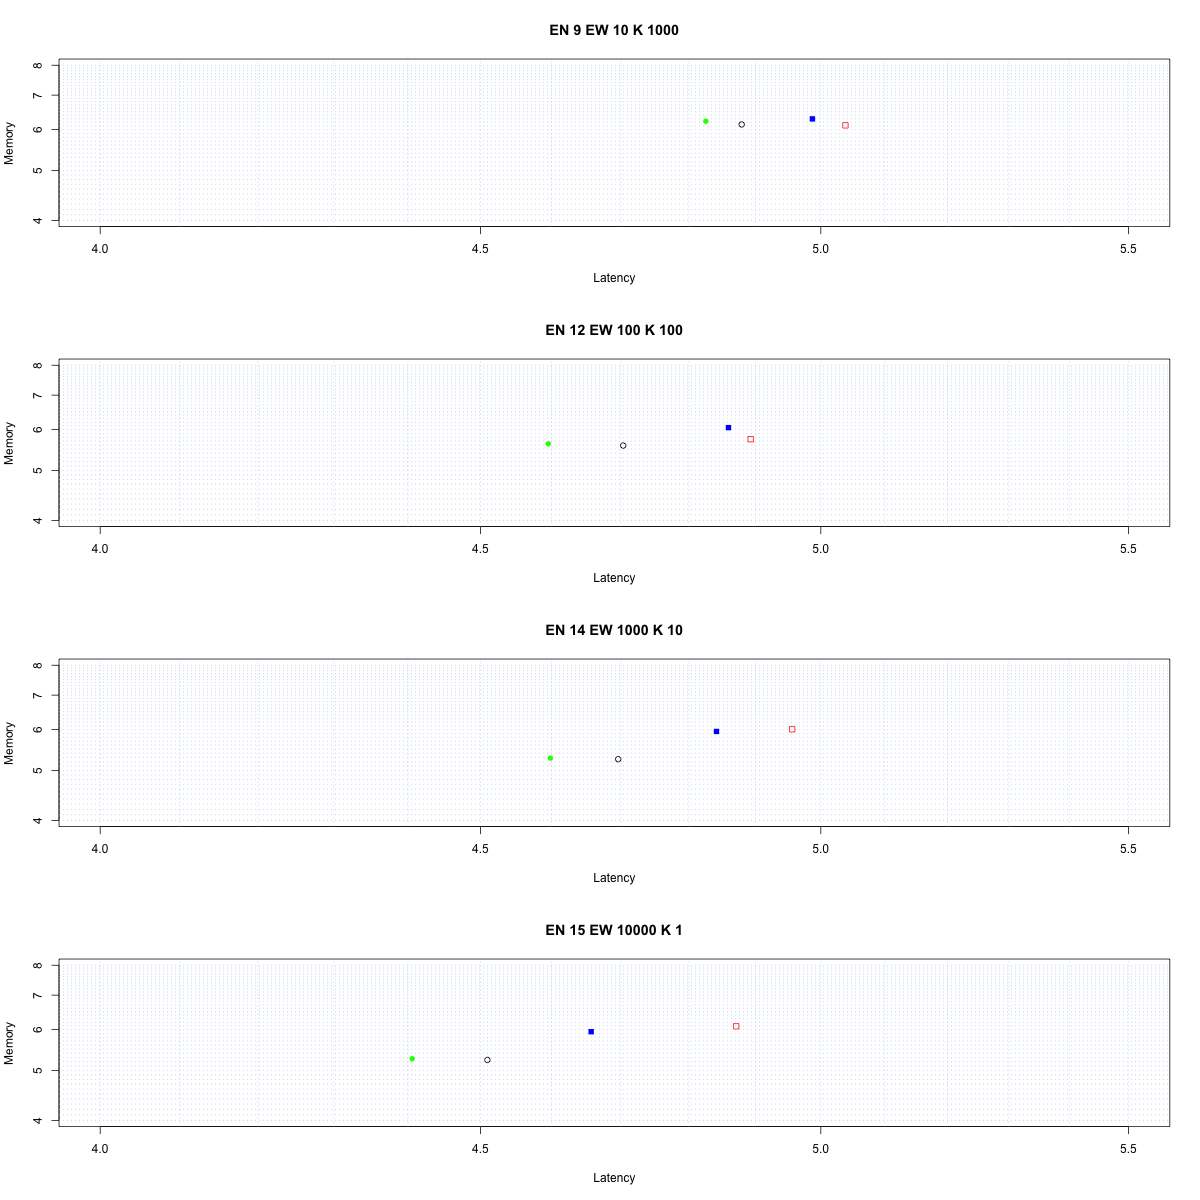
\includegraphics[width=0.90\linewidth]{images/dashboard-3-split}	
	\caption{Dashboard Three - $EW*K=10000$ Split} 
	\label{fig:result_dashboard_proba}
\end{figure}
\begin{figure}[tbh]
	\centering
	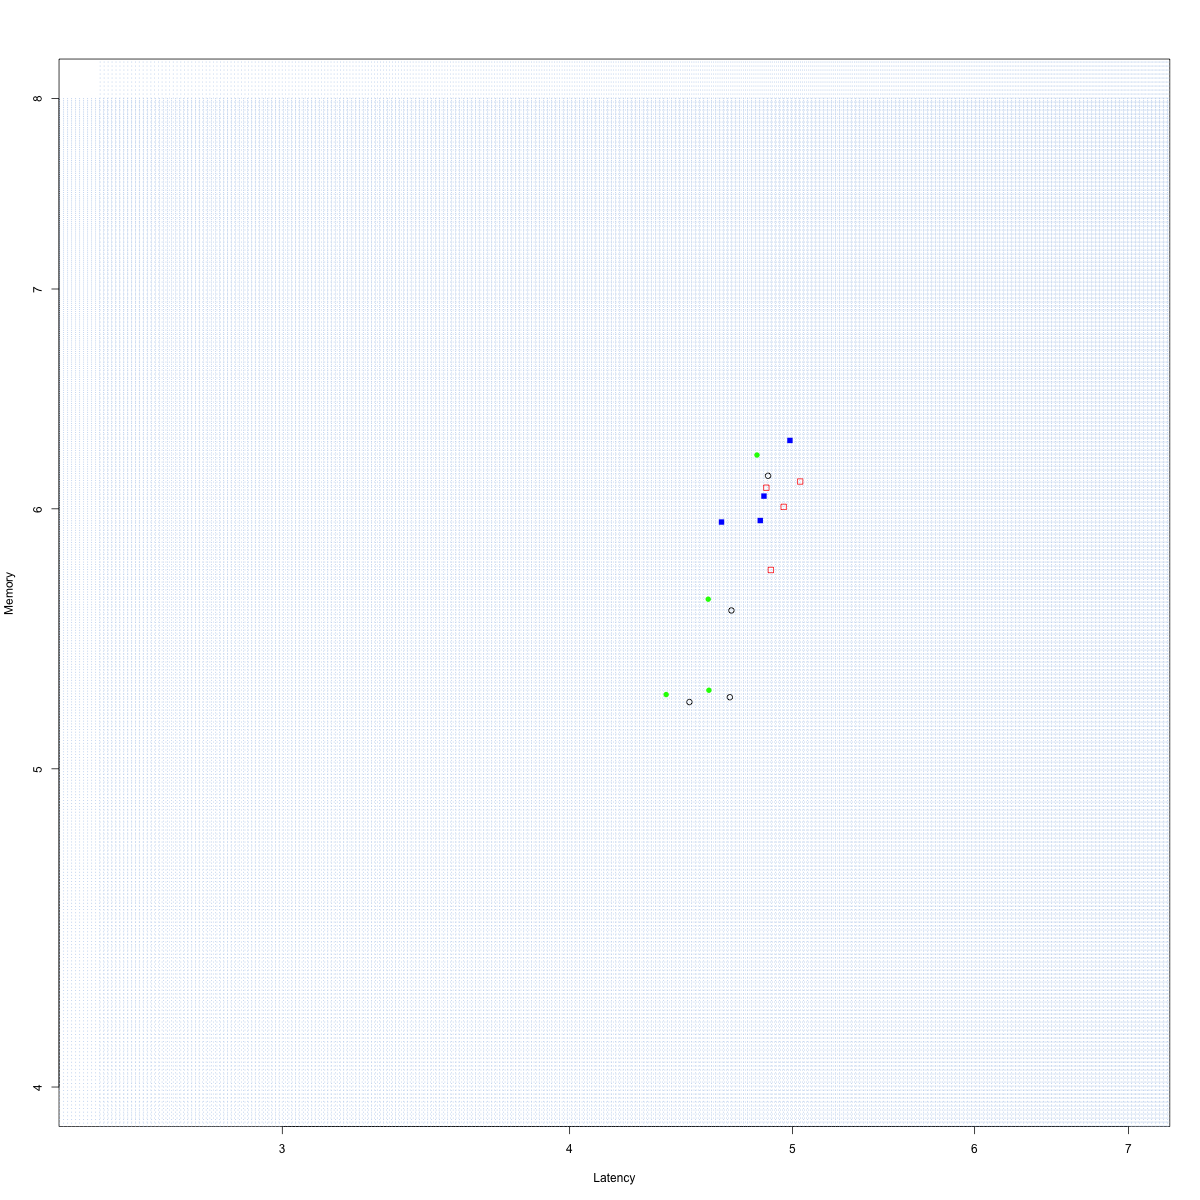
\includegraphics[width=0.90\linewidth]{images/dashboard-3}	
	\caption{Dashboard Three - $EW*K=10000$ Multiplot} 
	\label{fig:result_dashboard_probb}
\end{figure}

Figure \ref{fig:result_dashboard_proba}  shows how the behaviour of the four Baselines changes between a set of experiments which has a constant number triples within the active window equal to 10000, stated by maintaining the product CTEvent size (K) and Slot Number (EW) constant to 10000 triple. Fixing the window size in terms of triple to 10000 means moving form the left to the right on the lowest row of Table \ref{tab:soaktests-alt}. 

The main observation we can state on Figures \ref{fig:result_dashboard_proba} and \ref{fig:result_dashboard_probb}  is that the baselines performances seems depends only on the dimension of the active windows, indeed they are almost the same for all the compared experiments.

[Hp.1] is confirmed for both the memory and the latency as the figures show. However the difference are very small between the approaches. [Hp.2] is confirmed again observing a single reasoning approach at time, while in general it is not possible to say that Triple-based RDF Stream perform better than the Graph-based one.

Level 0 allows to state is there is no strong dominance of a Baseline w.r.t. the other ones in the provided analysis. Moreover, a week dominance can be observed in different steps both in term for Latency  and memory. The most clear example is in Figures \ref{fig:result_dashboard_ka} and \ref{fig:result_dashboard_kb} and in Figures \ref{fig:result_dashboard_ewa} and \ref{fig:result_dashboard_ewb} for medium size problems. However, result hierarchy is not absolute and it may changes by changing experiment configurations. This observation refutes explicitly HP.2 formulated in Section \ref{sec:soak-es}, while HP.1 was not completely confirmed. There are experiments where the naive  reasoning  approach seems performing better than the incremental one, at least in term of Latency. 

The research over RSP Engines requires further analysis at deeper levels to  motivate these unexpected findings and \name makes this possible.

\subsection{Level 1 -  Statistical Values Comparison}\label{sec:eval-level1}



The Analysis Level 1 exploits statistical investigation trough an easy to ready result layout, which simplify the inter-experiment comparison (see \ref{sec:analyser} Level 1)

The current evaluation operates over the mean values of Latency and Memory. Tables \ref{tab:soak_latency_comparisons} and \ref{tab:soak_memory_comparisons} constains in all the experiment results respectively for Latency and Memory.  Both the Tables dispose the result according with the layout of Table \ref{tab:soaktests-alt}. We decide to present only qualitative result representation, but \name allows also more detailed analysis with quantitative comparisons as shows in Section \ref{sec:analyser-impl}.

The results in Table \ref{tab:soak_latency_comparisons}.b and Table \ref{tab:soak_latency_comparisons}.d when N=1, i.e., the window contains only one \textit{CTEvent}, allow to state for large events that the Naive approach is faster than the Incremental one. Instead, when \textit{CTEvent} contains only few triples, the Incremental approach is faster. This is in contrast with [Hp.1] and moreover it is not intuitive and, because from theory we know that the incremental maintenance is more computationally expensive then materialisation for large changes \cite{DellAglio2014,DBLP:conf/cikm/RenP11,DBLP:conf/semweb/UrbaniMJHB13}. 

When $N>$1, the results in Table \ref{tab:soak_latency_comparisons}.a and \ref{tab:soak_latency_comparisons}.c allow to say that using a Triple-base RDF stream is faster than Graph-based one. This is because the graph data structure may speed up reasoning when it contains multiple triple, but it does so introducing an overhead that may hinder performances when it contains few triples \cite{DBLP:conf/semweb/BalduiniVDTPC13}. In particular, for the case $N$=1000 when the window contains 1000 triples (i.e., each \textsc{CTEvent} contains only one triple),  the Naive Triple-based approach is about 10\% faster  than the Naive Graph-based one while the Incremental Graph-based is even about 20\% faster. This findings partially confirm [Hp.2].

Finally, the results in Table \ref{tab:soak_latency_comparisons}.b and \ref{tab:soak_latency_comparisons}.d supports the idea that when the number of changing triples in $\Delta+ \Delta-$ (Section \ref{sec:baselines}) is a small fraction of those in the window an Incremental approach is faster than the Naive one as [Hp.1] states \cite{DellAglio2014,DBLP:conf/cikm/RenP11,DBLP:conf/semweb/UrbaniMJHB13}. The exception of the case $N$=1, but it can be seen as a limit case, where the reasoner is asked to deduce all the implicit triples implied by the only explicit triple in the window.  

While is possible to state meaningful observation over latency data, the same is not possible for memory ones. \name shows that the study of the memory can not be faced with the same methods to study latency (comparison of the mean values under a clearly identified the Steady State condition). 

Table \ref{tab:soak_memory_comparisons} reports the results for the memory usage during the experiments. Table entries do not confirm the what we observed in Table \ref{tab:soak_latency_comparisons} and sometimes it even refutes our findings. It is clear that memory usage does not follow the same behaviour of Latency, even if [Hp.1] and [Hp.2] are not totally refused by the results.

Further statistical analysis a surely meaningful. Maximum and minimum comparison within the same layout may detail much more the the system memory usage. However, trough \name is possible to lead the analysis to another level, observing the directly the memory usage in the time domain or in the frequency domain over all the experiment execution. 


\begin{table}[htbp]
	\centering
	\scriptsize
	\subtable[Incremental]{%
		\begin{tabular}{l | ccccc} % creating eight columns
	  	\hline
		Triple  & \multicolumn{5}{c}{Slots}  \\
		in & \multicolumn{5}{c}{Number}  \\
		Window  & 1 & 10 & 100 & 1000&10000\\
		\hline
		1	&G	\\			
		10	&G	&G	\\		
		100	&G	&G&	$\simeq$\\	
		1000&	G	&G	&$\simeq$&$\simeq$\\
		10000	&NA	&T	&S&	T	&T\\
		\hline % inserts single-line
	 \end{tabular}
	}
	\subtable[Triple]{%
		\begin{tabular}{l | ccccc} % creating eight columns
	  	\hline
		Triple  & \multicolumn{5}{c}{Slots}  \\
		in & \multicolumn{5}{c}{Number}  \\
		Window  & 1 & 10 & 100 & 1000&10000\\
		\hline
		1	&I	\\			
		10	&I	&I	\\		
		100	&N	&I&	I	\\	
		1000&	N&	I	&I	&I\\	
		10000&	NA	&I	&I	&I	&I\\
		\hline % inserts single-line
		\end{tabular}
	}	
	\subtable[Naive]{%
		\begin{tabular}{l | ccccc} % creating eight columns
	  	\hline
		Triple  & \multicolumn{5}{c}{Slots}  \\
		in & \multicolumn{5}{c}{Number}  \\
		Window  & 1 & 10 & 100 & 1000 &10000\\
		\hline
		1	&$\simeq$\\				
		10	& 	$\simeq$&	G	\\		
		100	&G	& 	$\simeq$&	T\\		
		1000	&G	&G	&T	&T	\\
		10000	&NA	& 	$\simeq$	& 	$\simeq$	&T	&T\\
		\hline % inserts single-line
	 	\end{tabular}
	}
	\subtable[Graph]{%
		\begin{tabular}{l | ccccc} % creating eight columns
	  	\hline
		Triple  & \multicolumn{5}{c}{Slots}  \\
		in & \multicolumn{5}{c}{Number}  \\
		Window  & 1 & 10 & 100 & 1000 &1000\\
		\hline			
		1	&I	\\			
		10	&I	&I		\\	
		100	& $\simeq$	&I	&I		\\
		1000 &	N	&I	&I	&I	\\
		10000&	NA	&I	&I	&I	&I\\
		\hline % inserts single-line
		\end{tabular}
	}
	\caption{(a), (c) - latency results comparison between Incremental and Naive approaches; (b), (d) - results comparison between Graph-based and Triple-based models}
	\label{tab:soak_latency_comparisons}	
\end{table}

				


\begin{table}[htbp]
	\centering
	\scriptsize
	\subtable[Incremental]{%
		\begin{tabular}{l | ccccc} % creating eight columns
	  	\hline
		Triple  & \multicolumn{5}{c}{Slots}  \\
		in & \multicolumn{5}{c}{Number}  \\
			Window  & 1 & 10 & 100& 1000&10000\\
		\hline
		1  	 & T\\
		10   & G     &  	T  \\
		100   & G     & 	T  & G\\
		1000& G     & 	\underline{G}  & G & T\\
		10000 &NA     & G  & G & G&G\\
		\hline % inserts single-line
	 \end{tabular}
	}
	\subtable[Triple]{%
		\begin{tabular}{l | ccccc} % creating eight columns
	  	\hline
		Triple  & \multicolumn{5}{c}{Slots}  \\
		in & \multicolumn{5}{c}{Number}  \\
			Window  & 1 & 10 & 100& 1000&10000\\
		\hline
		1    & N\\
		10   & I   & N \\
		100   & N & N & I\\
		1000 & N & I & I & I\\
		10000 & NA & I & I & I & I\\
		\hline % inserts single-line
		\end{tabular}
	}	

	\subtable[Naive]{%
		\begin{tabular}{l | ccccc} % creating eight columns
	  	\hline
		Triple  & \multicolumn{5}{c}{Slots}  \\
		in & \multicolumn{5}{c}{Number}  \\
			Window  & 1 & 10 & 100& 1000&10000\\
		\hline
		1  	 & G\\
		10   & G&  	T \\
		100   & G  & 	G  & T\\
		1000 & G& 	G & G & T\\
		10000 &  NA    & 	G  & 	G & T&T\\
		\hline % inserts single-line
	 	\end{tabular}
	}
	\subtable[Graph]{%
		\begin{tabular}{l | ccccc} % creating eight columns
	  	\hline
		Triple  & \multicolumn{5}{c}{Slots}  \\
		in & \multicolumn{5}{c}{Number}  \\
		Window  & 1 & 10 & 100& 1000&10000\\
		\hline
		1    & N\\
		10   & N   & N \\
		100& $\simeq$   & N & I \\
		1000& $\simeq$  & I & I & I \\
		100000  & NA & N & I & I & I \\
		\hline % inserts single-line
		\end{tabular}
	}	
	\caption{(a), (c) - memory results comparison between Incremental and Naive approaches; (b), (d) - results comparison between Graph-based and Triple-based models}
	\label{tab:soak_memory_comparisons}	
\end{table}


\subsection{Level 2 - Patter Identification}\label{sec:eval-level2}

Statistical analysis are meaningful, but may reduce to much the RSP Engine complexity by focusing on single element of comparison. A more complete analysis is required and \name can deepen trying to study the behaviour of the system over all the experiment execution.

Level 2 exploits again the layout of Table \ref{tab:soaktests-alt}, disposing in table cell a graphical representation of a certain variable (Latency, Memory). Which graphical representation use depends on the research necessities: time domain representations and value distribution are the ones we explored during our evaluation, both in log scale or linear scale.

\begin{figure}[hbt]
  \centering
	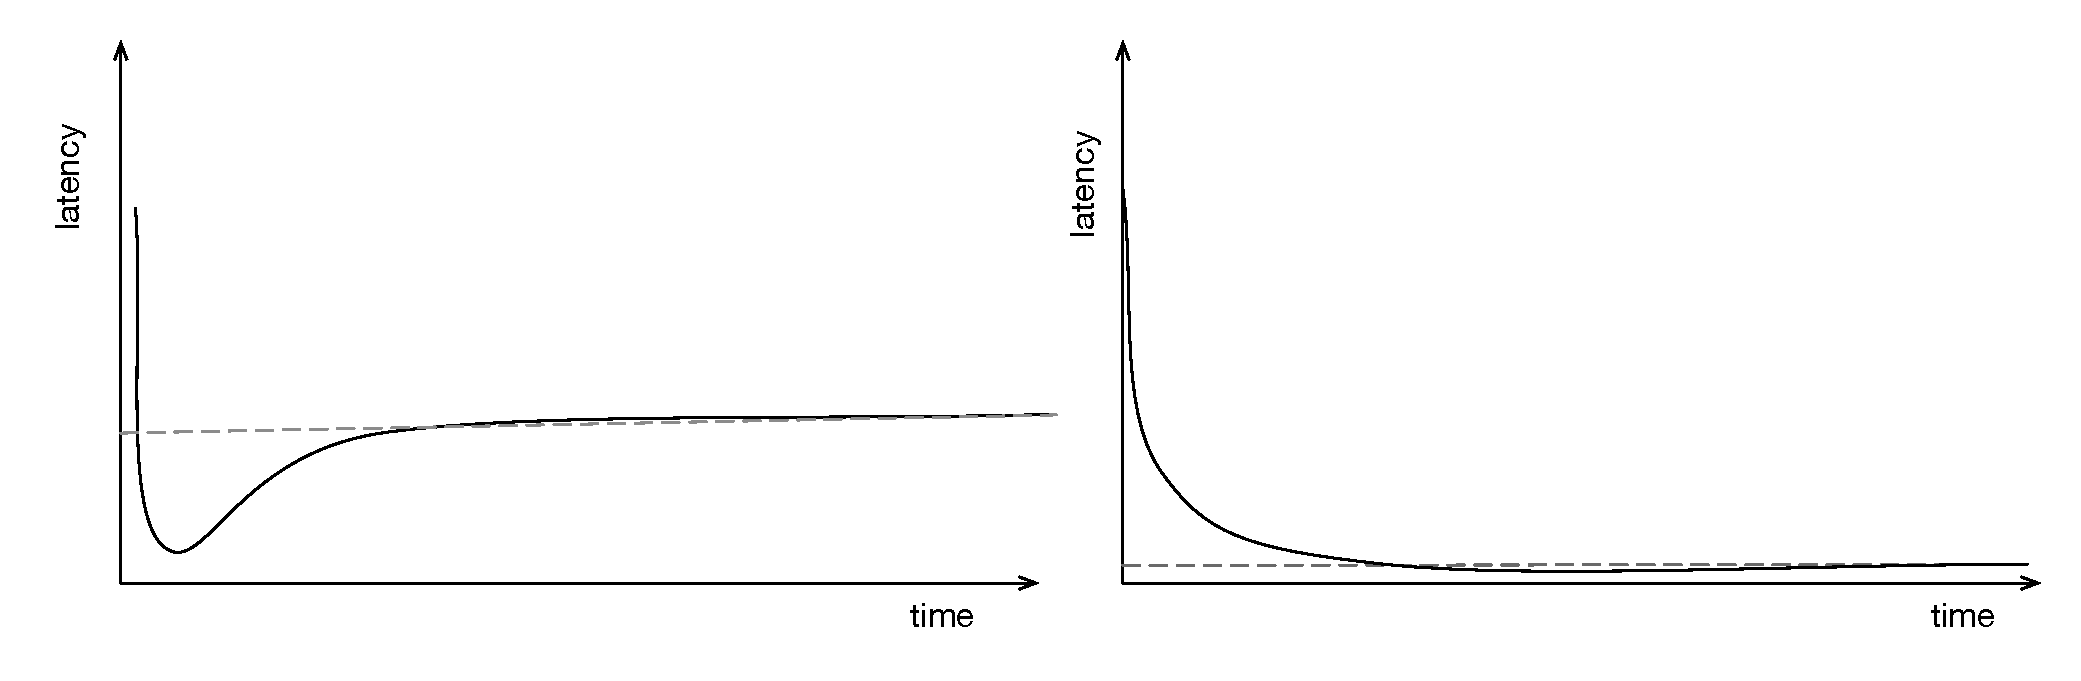
\includegraphics[width=\linewidth]{images/level2-pattern}
	\caption{Recognised Latency Pattern for SOAK Experiments} 
  	\label{fig:level2-pattern}
\end{figure}

The Figures \ref{fig:level2-latency-graph} and \ref{fig:level2-latency-triple} show the representation in linear scale of the Latency Time Series of the four Baselines. Immediately we can see that most of the systems reach a Steady State condition in a short period, between the 10\% and the 20\% of the entire experiment duration. Some of them show filling phenomena, when the sizes of the window start to be relevant w.r.t. the experiment duration. In general Latency trend follows one of the pattern showed in Figure \ref{fig:level2-pattern}. %Moreover, the responsiveness is not guaranteed for the biggest experiments, especially during the warm-up phase.

The Figures \ref{fig:level2-memory-graph} and \ref{fig:level2-memory-triple} represent the  representation in linear scale of the Memory Time Series of the four Baselines. We can observe that, despite what happens for latency, memory usage does not reach a Steady State condition for all the experiments (Baseline GI and TI for Windows of dimension 1000 Triples with more than one slot).  When it is reached, the Steady State condition requires form 10\% to 80\% of the entire experiment duration, and in general it has not a common behaviour for many experiments. The variance of these results is high, and can be motivated arguing about how Java is managing the memory during the execution. The optimisation policies work better when the system have to handle a lot of triples. The proof of this insight can be seen in Figures \ref{fig:level2-memory-graph} and \ref{fig:level2-memory-triple}, where the lower levels reach the Steady State condition before the higher ones, which actually does not reach the Steady State at all for some Experiment with GI and TI.  For very small problems with the Incremental Approach, the Steady State is not even reached, maybe because the memory consume does not alert the JVM at all. 
The filling phenomena we identified for latency are still visible in both the figures This denotes the existence of a relation exists between memory. This is one of the point we can further investigate trough the next analysis step: Level 3.

Figures \ref{fig:level2-memory-density-graph} and \ref{fig:level2-memory-density-graph} represent the distribution of Memory Time Series values of the four Baselines. To obtain this representation we individuate the minimum and the maximum between all the experiments. We divided the span in ten intervals and automatically we count ho many values of the Memory time series fit the intervals, repeating this count for all the experiment. Trough this representation we can see how the memory usage is distributed during the experiment execution. Firstly we can observe that the memory has a "Gaussian" distribution, which variances is lower for baselines GI and TI, which exploit incremental reasoning and thus have a smarter usage of the memory. When the window size increases, the memory consumption shift to the right, towards the intervals with higher values too.

All the four Figures about Memory Time Series and Memory distribution show that there are strong difference between the experiment subset with Window dimension of 1000 and the ones with window dimension 10000. This is a meta-insight that improve the Experiment Design model, stating that there we are still not able to predict the baselines behaviour, but we can further investigate trough \namens.

The quantitative nature of the hypothesis formulated in Section \ref{sec:soak-es} does not allow to exploit Level 3 for Hypothesis verification. Actually [Hp.1] and [Hp.2] consider the performance as the main evaluation metric, while Level 2 fulfils the necessity to understand the system nature. The insights above allow to improve the RSP Engine model, upon which is possible to formulate more precise hypothesis and to explain the unpredictable results we obtained from Level 0 and Level 1.

\begin{figure}[hbt]
  \centering
	\includegraphics[width=\linewidth]{images/lat-log-graph}
	\caption{The Linear Representation Scale of the Latency Time Series for GN and GI} 
  	\label{fig:level2-latency-graph}
\end{figure}

\begin{figure}[hbt]
  \centering
	\includegraphics[width=\linewidth]{images/lat-log-triple}
	\caption{The Linear Representation Scale of the Latency Time Series for TN and TI} 
  	\label{fig:level2-latency-triple}
\end{figure}


\begin{figure}[hbt]
  \centering
	\includegraphics[width=\linewidth]{images/mema-graph}
	\caption{The Linear Representation Scale of the Memory Time Series for GN and GI} 
  	\label{fig:level2-memory-graph}
\end{figure}

\begin{figure}[hbt]
  \centering
	\includegraphics[width=\linewidth]{images/mema-triple}
	\caption{The Linear Representation Scale of the Memory Time Series for TN and TI} 
  	\label{fig:level2-memory-triple}
\end{figure}

\begin{figure}[hbt]
  \centering
	\includegraphics[width=\linewidth]{images/mema-dens-graph}
	\caption{GN and GI Distribution of Memory Time Series Values over 10 Intervals between the Minimum to the Maximum over all the Experiments} 
  	\label{fig:level2-memory-density-graph}
\end{figure}

\begin{figure}[hbt]
  \centering
	\includegraphics[width=\linewidth]{images/mema-dens-triple}
	\caption{TN and TI Distribution of Memory Time Series Values over 10 Intervals between the Minimum to the Maximum over all the Experiments} 
  	\label{fig:level2-memory-density-triple}
\end{figure}

\subsection{Level 3 - Single Visual Comparison}\label{sec:eval-level3}
	
Level 2 has shown some macroscopic differences between the all the experiments, which can explain the absence of a dominant solution over all the experiment w.r.t [Hp.1] and [Hp.2]. Level 3 operates a drill down from Level 2. For this evaluation we provide examples of intra experiment analysis. Our goals is understand the relation between Memory and Latency, with the aim to understand what influence the performances. For this reason, even if at Level 3 it is possible also to provide inter-experiment comparison (see Section \ref{sec:analyser}) for soak test we only exploit multivarible comparison within an experiment.

Level 2 has pointed out three important findings:
\begin{itemize}
\item Despite all the experiment reach a Steady State condition for latency, some of does not reach it for memory.
\item When the Steady State condition is reached, form memory it required 10-20\% of the total experiment duration, while for memory it necessities of 30-70\% of the total number of streamed events.
\item Filling phenomena can be identified for both memory and latency and my be further investigate trough direct comparisons.
\end{itemize}

Figure \ref{fig:level3-not-steady-naive-graph-en11} contains two examples of experiment that reach the Steady State condition for latency but not for memory. Figure \ref{fig:level3-not-steady-naive-graph-en11}.a shows the latency and memory usage for the Baseline GN within the experiment eleven (\textsc{CTEvent} size = 10, Number of Slot = 100), Figure \ref{fig:level3-not-steady-naive-graph-en11}.b shows within the same experiment the latency and memory usage of the Baseline TI. 

If we consider only the memory trend, we note an oscillating behaviour which contrast with the idea of Steady State. A more careful analysis identifies the presence of some spikes in the latency time series, which represent a certain period of time where the content of the window requires a strong reasoning effort, which may also influence the memory usage. Moreover, This kind of analysis can not be seen form higher level. 

\begin{figure}[tbh]
  \centering
  \subfigure[GN Exp 11, \textsc{CTEvent} Size = 10 Num.Slot = 100]{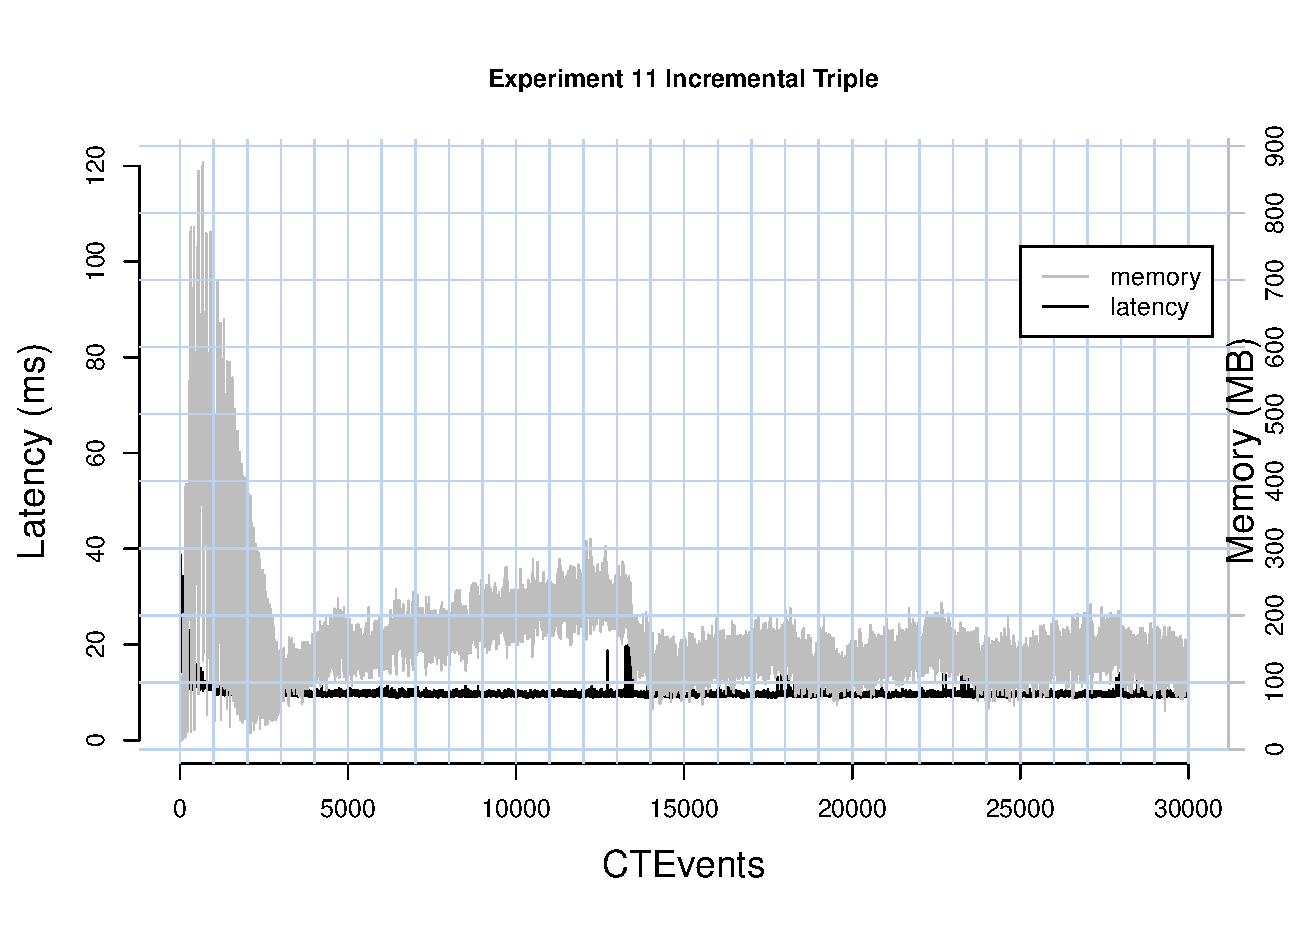
\includegraphics[width=0.40\linewidth]{images/level3-not-steady-naive-graph-en11}}
  \subfigure[TI Exp 11, \textsc{CTEvent} Size = 10 Num.Slot = 100]{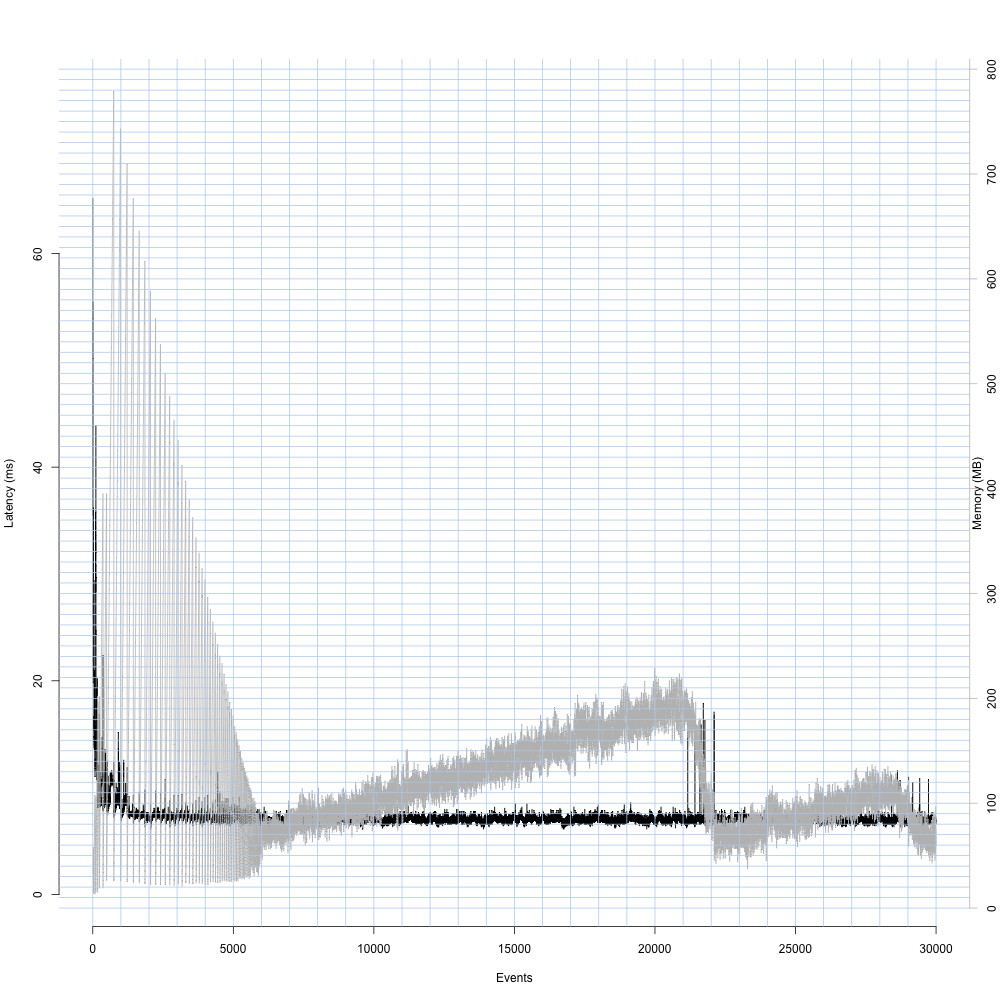
\includegraphics[width=0.40\linewidth]{images/level3-not-steady-inc-stmt-en11}}
  \caption{Comparison between memory and latency on difference in Steady State condition reaching} 
  \label{fig:level3-not-steady-naive-graph-en11}
\end{figure}

Figure \ref{fig:level3-steady-naive-graph-en7-12} shows two examples of steady state condition reaching. The subfigure (a) describes that the Baseline GN for experiment seven (\textsc{CTEvent} size = 10, Number of Slot = 10) reaches the Steady State around the 10\% of the entire experiment duration for latency and about 45\% for memory. The only observation we can point out is that Java improve the performances first to execute faster then to save resources. A completely different behaviour can be appreciate in the subfigure (b), where both latency and memory reach the Steady State around the 10\% of the entire execution. It seems that bigger is the amount of resources required by the program, faster Java optimization policies work.


\begin{figure}[tbh]
  \centering
  \subfigure[GN Exp 7, \textsc{CTEvent} Size = 10, Num.Slot = 10]{
	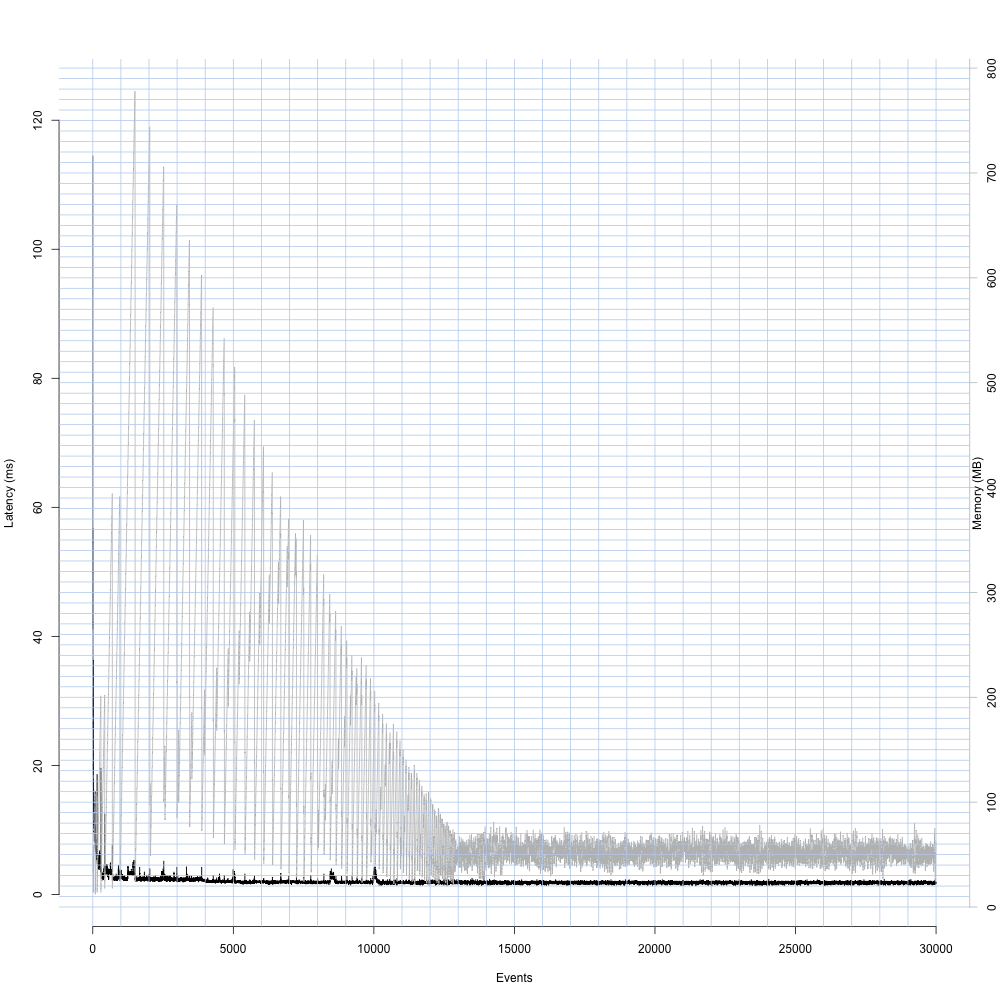
\includegraphics[width=0.40\linewidth]{images/level3-steady-naive-graph-en7}
	}
	\subfigure[GI Exp 12, \textsc{CTEvent} Size = 100, Num.Slot = 100]{
	  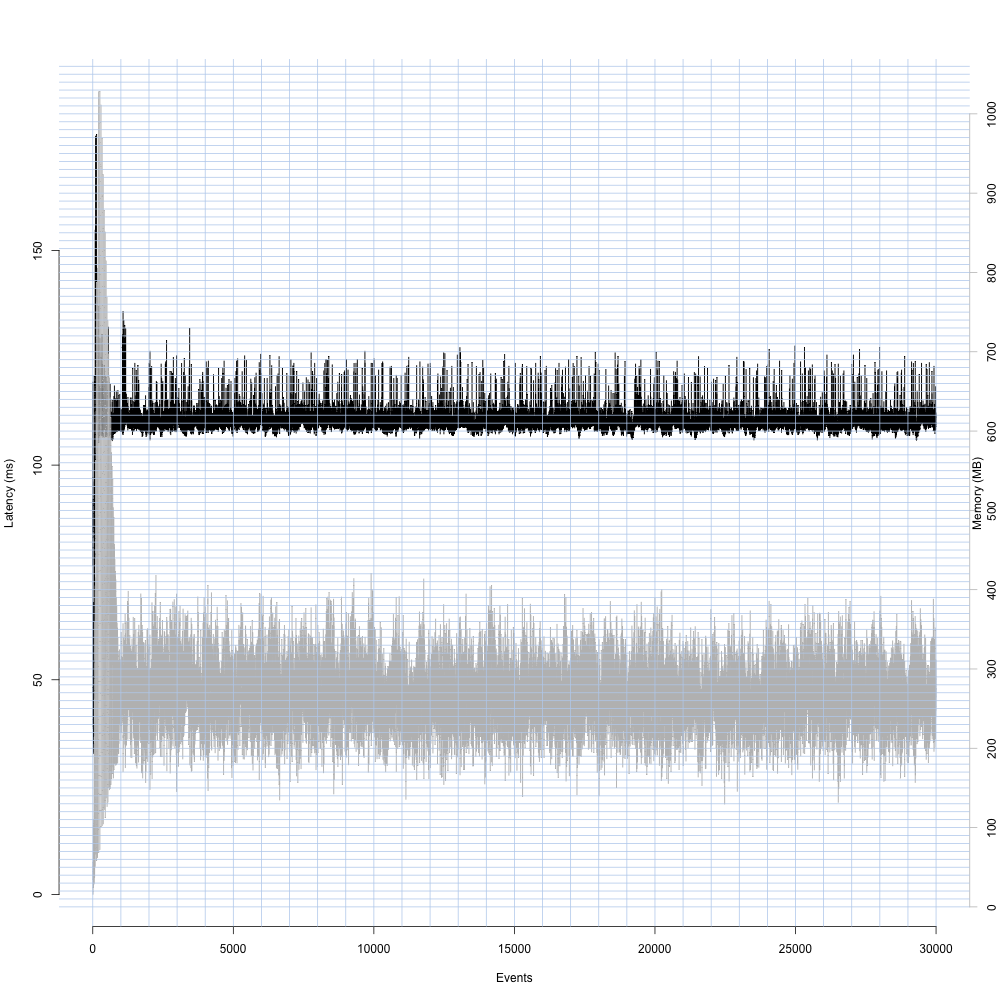
\includegraphics[width=0.40\linewidth]{images/level3-steady-inc-graph-en12}
	}
  	\label{fig:level3-steady-naive-graph-en7-12}  	
  	\caption{Comparison of steady state condition reaching between latency and memory} 
\end{figure}

Figures \ref{fig:level3-filling-inc-stmt-en15} (a) and (b) show the relation between the filling phenomena together for latency and memory for the Baselines TN and TI within Experiment fifteen ( \textsc{CTEvent} size = 1 Number of Slot = 10000). Independently from which baseline we observe, the main insight regards how Java manages the initial warm-up phase. As we seen in other experiments it starts allocating an excessive amount of memory, which it immediately tries to reduce. The different with other experiment is that the window dimension is increasing and thus the amount of memory occupation. The system worsening in term of latency follows the increasing memory usage. Finally, when Java has evaluated the correct (stable) amount of memory to handle the active window, the latency and reaches the stability too.

\begin{figure}[tbh]
  \centering
  \subfigure[TN Exp 15, \textsc{CTEvent} Size = 1 Num.Slot = 10000]{
	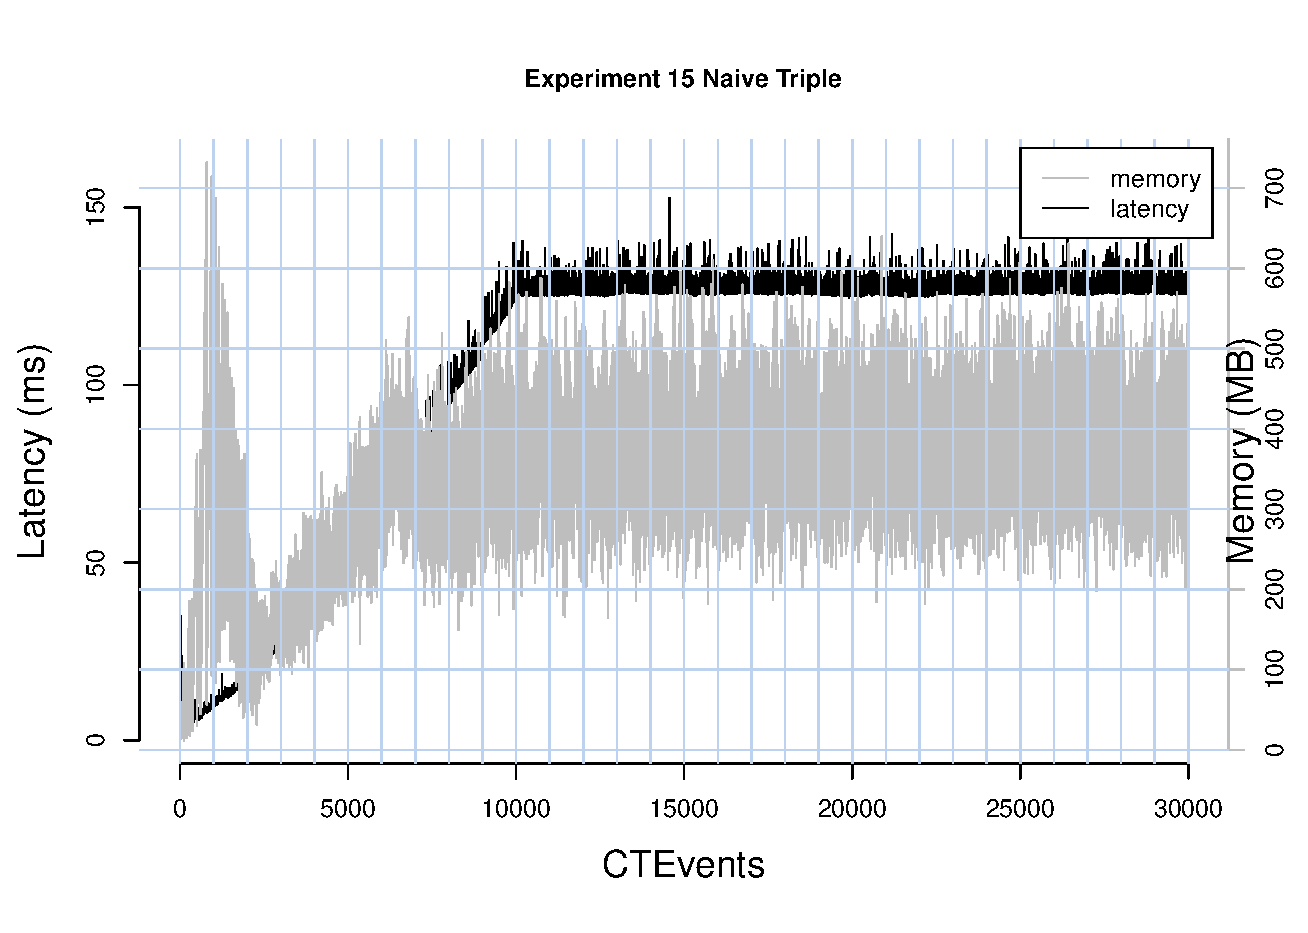
\includegraphics[width=0.40\linewidth]{images/level3-filling-naive-stmt-en15}
	}
\subfigure[[TI Exp 15, \textsc{CTEvent} Size = 1 Num.Slot = 10000]{
	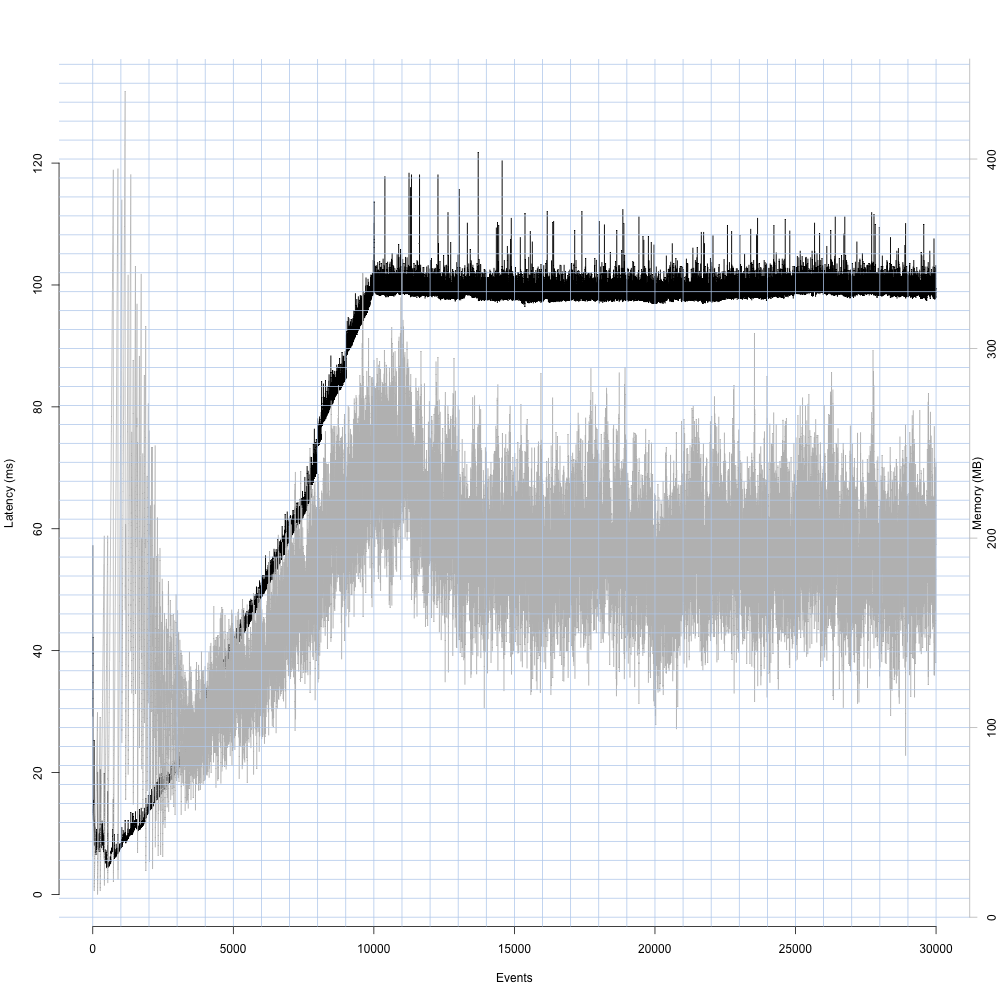
\includegraphics[width=0.40\linewidth]{images/level3-filling-inc-stmt-en15}
	}
	\caption{Comparison of filling phenomena between latency and memory} 
  	\label{fig:level3-filling-inc-stmt-en15}
\end{figure}


\section{StepResponse Test Evaluation Results}\label{sec:stressres}
 Finally we show \name abilities presenting the results of Step Response tests in the Subsection \ref{sec:stressres}.


